\subsection{Abstraction Levels}
Code analysis is performed on three different abstraction levels.
\newline
The first level is the original dex bytecode contained in the \textit{classes.dex}.
As will be shown chapter~\ref{chapter:luckypatcher}, it is target of the attack.
\newline
The second level is the smali code.
It is used to represent the dex bytecode in a readable way and to identify the result of the changes.
\newline
The third level is the Java code.
It is the best presentation to interpret and understand the changes in the context of methods or classes.
\newline
The Java code can be decompiled from the dex bytecode since the build process can be reversed as seen in figure~\ref{fig:re1}.
\begin{figure}[h]
    \centering
    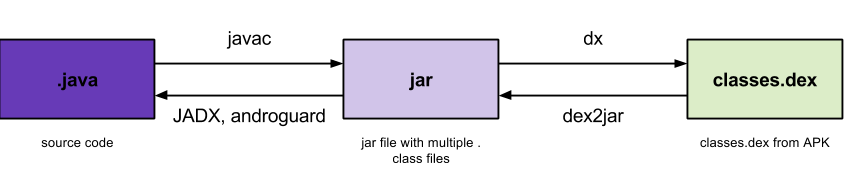
\includegraphics[width=1\textwidth]{data/re1.png}
    \caption{Bidirectional relation between Java .class and .dex bytecode \cite{andevconDalvikART}}
    \label{fig:re1}
\end{figure}

\subsubsection{dex Analysis} \label{subsection:tools-dex}
The \textit{classes.dex} contains the application code and has to be modified by the cracking tool to carry out the attack.
Analysing the dex bytecode allows to point out the places in the bytecode that have been modified.
\newline
The extraction of the \textit{classes.dex} is done using a simple script shown in code snippet~\ref{codeSnippet:dexScript}.
\newline
\lstinputlisting[
  float=h,
  breaklines=true,
  captionpos=b,
  frame=single,
  numbers=left,
  language=bash,
  linerange={32-35},
  firstnumber=1,
  caption={Script to extract the \gls{dex} bytecode from the \gls{apk}},
  label={codeSnippet:dexScript}
]{data/extractScript.sh}
The \gls{apk} is an archive file and can be unpacked using \textit{unzip}.
The content is unpacked to the destination which is added with the parameter \textit{-d destination} as seen in line 3.
The extracted \textit{classes.dex} contains the code in binary.
Hexdump is used to convert the code into a hexadecimal view.
\newline
The output contains the line number, the bytecode and the ASCII translation.
Code snippet~\ref{codeSnippet:dexOutput} is an example of the beginning of the \textit{classes.dex} file.
In this view, one character is 4 bit, thus one tuple is one byte and two bytes form a 16 bit opcode.
This presentation allows to better identify opcodes and translate them using an opcode table \cite{opcodes}.
For example, the first 8 byte or 16 hex tuples, \textit{64 65 78 0A 30 33 35 00}, are the \gls{dex} file magic, which identifies the file type.
Translated to ASCII, the result is \textit{dex.035.}.
\begin{lstlisting}[
  float=h,
  basicstyle=\ttfamily\small,
  breaklines=true,
  captionpos=b,
  frame=single,
  caption={Hexadecimal view of classes.dex},
  label={codeSnippet:dexOutput}
]
00000000  64 65 78 0a 30 33 35 00  ae a5 51 7e 06 f7 00 84  |dex.035...Q~....|
00000010  ee 23 5d 3b 4a 61 bb 08  51 a7 c9 02 c1 4e d2 91  |.#];Ja..Q....N..|
00000020  0c fb 21 00 70 00 00 00  78 56 34 12 00 00 00 00  |..!.p...xV4.....|
00000030  00 00 00 00 ac 88 06 00  f4 4e 00 00 70 00 00 00  |.........N..p...|
00000040  ad 09 00 00 40 3c 01 00  0a 0e 00 00 f4 62 01 00  |....@<.......b..|
00000050  3d 27 00 00 6c 0b 02 00  ff 4b 00 00 54 45 03 00  |='..l....K..TE..|
\end{lstlisting}
\newline

\subsubsection{Smali Analysis} \label{subsection:tools-baksmali}
The smali code is disassembled from dex bytecode using \textit{baksmali} \cite{smali}.
This is done in order to interpret the changes in the bytecode regarding functionality.
\newline
Assembling and disassembling of dex and smali is possible without the loss information since they have a bijective mapping\cite{smali}.
The syntax is loosely based on the Jasmin syntax \cite{smali}.
Smali takes the \gls{apk} and disassembles its \textit{classes.dex} file.
The output is a smali file for each class.
Smali has two advantages over dex bytecode.
The first advantage is the replacing of opcodes with their actual opcode name.
The second advantage is the reconstruction of the class and method structure.
This makes it easier to analyse the code.
This process is done using the script in code snippet~\ref{codeSnippet:smaliScript}.
\newline
\lstinputlisting[
  float=h,
  breaklines=true,
  captionpos=b,
  frame=single,
  numbers=left,
  language=bash,
  linerange={19-21},
  firstnumber=1,
  caption={Script to generate the corresponding smali code for a given \gls{apk}},
  label={codeSnippet:smaliScript}
]{data/extractScript.sh}
\newline
An example of smali code can be seen in code snippet~\ref{codeSnippet:smaliOutput}.
It is easier to understand than the dex presentation.
The content of variables, as in line 3, can be identified without big effort.
This enables the reader analyse the application's workflow similar to the source code.
\newline
\begin{lstlisting}[
  float=h,
  basicstyle=\footnotesize,
  breaklines=true,
  captionpos=b,
  frame=single,
  firstnumber=1,
  caption={Example of smali code},
  label={codeSnippet:smaliOutput}
]
# virtual methods
.method public magic()V
  const-string v4, "android_id"
  ...
  move-result v0
  if-eqz v0, :cond_7
  ...
.end method
\end{lstlisting}

\subsubsection{Java Analysis} \label{subsection:forensics-tools-java}
Java code suits best for the analysis of the new behavior since its presentation is close to the what people are programming.
It has names variable and method which makes it better understandable.
The representation is close to how the developer implemented the application.
\newline
As seen in figure~\ref{fig:re1}, the .dex files can be reengineered to Java \gls{classg} files.
The reengineered Java code maintains the semantics, but does not exactly match the source code.
As we will see, code attacked may contain instructions that are removed by the decompiler.
Sometimes a decompiler does not deliver an acceptable result, that is why DAD and JADX are used alternatively.
\newline
DAD, is a short name of "DAD is A Decompiler".
It is part of Androguard \cite{androguard}, a reverse engineering tool for Android.
It works with the dex bytecode and does not require third party tools like dex2jar \cite{dex2jar}.
Code snippet~\ref{codeSnippet:androguardScript} shows how it is used in the command line interface to decompile the \gls{apk} into Java code.
\newline
\lstinputlisting[
  float=h,
  breaklines=true,
  captionpos=b,
  frame=single,
  numbers=left,
  language=bash,
  linerange={7-9},
  firstnumber=1,
  caption={Script to decompile to Java using androguard},
  label={codeSnippet:androguardScript}
]{data/extractScript.sh}
\newline
JADX \cite{jadx} is the second decompiler.
The decompilation is directly done from the \gls{apk}'s dex bytecode to Java code and can be performed in the command line interface as seen in Code snippet~\ref{codeSnippet:jadxScript}.
\newline
\lstinputlisting[
  float=h,
  breaklines=true,
  captionpos=b,
  frame=single,
  numbers=left,
  language=bash,
  linerange={28-30},
  firstnumber=1,
  caption={Script to decompile to Java using JADX},
  label={codeSnippet:jadxScript}
]{data/extractScript.sh}
